\section{What \code{\_entities} Asks For}
\label{sec:ch11-what-entities-asks-for}
\index{\_entities@\code{\_entities}!how it resolves|(}%

Chapter~\ref{ch:the-first-cut-extracting-catalog} put a reference resolver on
\code{Product} in both services and asserted, in that chapter's own gate, that
twenty-five representations cost Catalog one statement. It did not say how, and
the how turns out to matter, because there is a way of writing the same
resolver that costs twenty-five.

\index{HotChocolate!EntitiesResolver@\code{EntitiesResolver}}%
The whole of the mechanism is one file in the HotChocolate source tree, read at
tag \code{16.6.0}, commit \code{8fea46e}:

\begin{minted}[fontsize=\scriptsize]{text}
src/HotChocolate/ApolloFederation/src/ApolloFederation/Resolvers/EntitiesResolver.cs
\end{minted}

It is two loops. The first walks the representations and, for
each one, finds the object type by its \code{\_\_typename}, checks that the
type carries a reference resolver, clones the resolver context, puts the type
and the representation into the clone's local state, and starts a task. It does
not await it. The comment in the source says why:

\begin{minted}[fontsize=\footnotesize,breaklines]{text}
// We clone the resolver context here so that we can split the work
// into subtasks that can be awaited in parallel and produce separate results.
\end{minted}

The second loop awaits those tasks in order and writes each result into an
array at the representation's own index.

\index{reference resolver!called once per representation}%
Three things follow from that, and the first is the one people get wrong.
\textbf{There is no batch-shaped entry point.} Your reference resolver is
called once per representation and never sees the list. Whatever batching you
get, you build.

\textbf{Every call is started before any of them is awaited.} That is the
condition a DataLoader needs. Twenty-five calls to \code{LoadAsync} enqueue
twenty-five keys before the first one blocks on a result, so one batch forms
and one query goes out.

\textbf{A failure belongs to its index.} The second loop looks at each task
twice over: a task that has already finished is inspected for an
\code{Exception} without being awaited, and one that has not is awaited inside
a \code{try}. Either way a failure writes null into that slot and reports an
error with the index appended to the path.
Section~\ref{sec:ch11-null-at-the-boundary} is about what a client makes of
that; here the point is only that the other twenty-four are unaffected.

\subsection*{Watching it happen}

\index{samples!entity-resolution@\code{entity-resolution}}%
Mosaic cannot show me any of this. Catalog has no request timeline, no resolver
count and no statement counter, because
chapter~\ref{ch:the-life-of-a-request} built the first two inside
\code{Mosaic.Api}, chapter~\ref{ch:data-without-the-n-plus-1} added the third
beside them, and
chapter~\ref{ch:the-first-cut-extracting-catalog}'s extraction left all three
there. Chapter~\ref{ch:enter-the-router} recorded that gap and
chapter~\ref{ch:observability} owns closing it properly, with tracing that
spans both services rather than a second copy of one chapter's diagnostic
listener.

So the mechanism gets a sample of its own, which is what this book does with
mechanisms. \code{samples/entity-resolution} has two subgraphs, named
\code{catalog} and \code{crates} inside the sample and nothing to do with
Mosaic's services of similar name. The first holds four widgets and two entity
types over them. \code{Widget} resolves through a DataLoader. \code{Gadget} is
the same entity with a resolver that fetches one key at a time, which is what a
subgraph looks like before anybody thinks about the batch. Both write a line to
a log the subgraph exposes as \code{Query.resolutionLog}, and so does the store
they read from.

Here is \code{Widget}, with its documentation comments taken out and nothing
else:

\begin{minted}[fontsize=\footnotesize,breaklines]{csharp}
[Key("id")]
public sealed class Widget
{
    [ID]
    public required string Id { get; init; }

    public required string Name { get; init; }

    [ReferenceResolver]
    public static async Task<Widget?> ResolveByIdAsync(
        string id,
        IWidgetByIdDataLoader widgetById,
        CancellationToken cancellationToken)
    {
        ResolutionLog.Write($"enter  Widget/{id}");
        var widget = await widgetById.LoadAsync(id, cancellationToken);
        ResolutionLog.Write($"leave  Widget/{id}");
        return widget;
    }
}
\end{minted}

\code{Gadget}'s is the same shape with one substitution: it takes the store
rather than the DataLoader, and asks it for one key rather than adding one to a
batch.

\index{\_entities@\code{\_entities}!four representations, one call}%
Four widgets in one \code{\_entities} call, and the log the subgraph wrote:

\begin{minted}[fontsize=\footnotesize]{text}
enter  Widget/w1
enter  Widget/w2
enter  Widget/w3
enter  Widget/w4
lookup 4 keys: w1, w2, w3, w4
leave  Widget/w4
leave  Widget/w3
leave  Widget/w2
leave  Widget/w1
entries: 4 on 1 thread(s)
\end{minted}

Four entries before the store is touched at all, then one journey for four
keys. The last line is derived rather than printed raw: the log records the
managed thread of every \code{enter} and reports how many distinct ones there
were, because a raw thread number would be a different number on every run.

Now the same four keys as gadgets:

\begin{minted}[fontsize=\footnotesize]{text}
enter  Gadget/w1
lookup 1 key: w1
leave  Gadget/w1
enter  Gadget/w2
lookup 1 key: w2
leave  Gadget/w2
enter  Gadget/w3
lookup 1 key: w3
leave  Gadget/w3
enter  Gadget/w4
lookup 1 key: w4
leave  Gadget/w4
entries: 4 on 1 thread(s)
\end{minted}

Figure~\ref{fig:ch11-batch-timeline} puts the two side by side, because the
difference is easier to see than to describe.

\begin{figure}[htbp]
  \centering
  % Four representations through a reference resolver, with a DataLoader behind
% it and without one. Referenced from chapter 11. Bare tikzpicture; the figure
% environment, caption and label live at the call site.
%
% The point of the picture is that the left column has one lookup and the right
% column has four, and that the reason is not the number of calls: both columns
% enter the resolver four times. What differs is whether the four calls are in
% flight at the same moment.
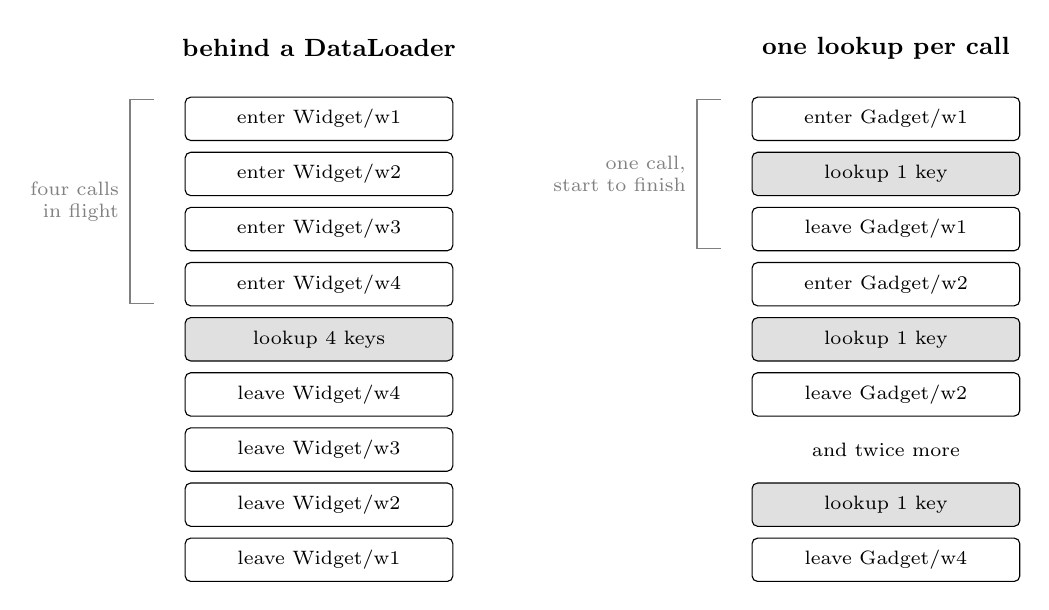
\begin{tikzpicture}[
    font=\small,
    head/.style={font=\small\bfseries, align=center},
    call/.style={draw, rounded corners=2pt, minimum width=34mm,
                 minimum height=5.5mm, align=center, font=\scriptsize},
    hit/.style={draw, rounded corners=2pt, minimum width=34mm,
                minimum height=5.5mm, align=center, font=\scriptsize,
                fill=black!12},
    span/.style={gray},
    lbl/.style={font=\scriptsize, align=center, inner sep=1pt}
  ]

  \node[head] at (2.6,0.6)  {behind a DataLoader};
  \node[head] at (9.8,0.6)  {one lookup per call};

  % -- left column: all four enter, then one lookup --------------------------
  \node[call] (l1) at (2.6,-0.3) {\code{enter  Widget/w1}};
  \node[call] (l2) at (2.6,-1.0) {\code{enter  Widget/w2}};
  \node[call] (l3) at (2.6,-1.7) {\code{enter  Widget/w3}};
  \node[call] (l4) at (2.6,-2.4) {\code{enter  Widget/w4}};
  \node[hit]  (lb) at (2.6,-3.1) {\code{lookup 4 keys}};
  \node[call] (l5) at (2.6,-3.8) {\code{leave  Widget/w4}};
  \node[call] (l6) at (2.6,-4.5) {\code{leave  Widget/w3}};
  \node[call] (l7) at (2.6,-5.2) {\code{leave  Widget/w2}};
  \node[call] (l8) at (2.6,-5.9) {\code{leave  Widget/w1}};

  \draw[span] (0.5,-0.05) -- (0.2,-0.05) -- (0.2,-2.65) -- (0.5,-2.65);
  \node[lbl, span, anchor=east, align=right] at (0.1,-1.35)
    {four calls\\in flight};

  % -- right column: enter, lookup, leave, four times ------------------------
  \node[call] (r1) at (9.8,-0.3) {\code{enter  Gadget/w1}};
  \node[hit]  (r2) at (9.8,-1.0) {\code{lookup 1 key}};
  \node[call] (r3) at (9.8,-1.7) {\code{leave  Gadget/w1}};
  \node[call] (r4) at (9.8,-2.4) {\code{enter  Gadget/w2}};
  \node[hit]  (r5) at (9.8,-3.1) {\code{lookup 1 key}};
  \node[call] (r6) at (9.8,-3.8) {\code{leave  Gadget/w2}};
  \node[lbl]        at (9.8,-4.5) {and twice more};
  \node[hit]  (r7) at (9.8,-5.2) {\code{lookup 1 key}};
  \node[call] (r8) at (9.8,-5.9) {\code{leave  Gadget/w4}};

  \draw[span] (7.7,-0.05) -- (7.4,-0.05) -- (7.4,-1.95) -- (7.7,-1.95);
  \node[lbl, span, anchor=east, align=right] at (7.3,-1.0)
    {one call,\\start to finish};

\end{tikzpicture}

  \caption{The same four representations, twice. Both columns enter the
  resolver four times, so the count of calls is not what separates them. On the
  left all four are in flight when the batch dispatches; on the right each call
  runs to completion before the next one starts, and the four tasks
  \code{EntitiesResolver} created were never concurrent for a moment.}
  \label{fig:ch11-batch-timeline}
\end{figure}

\index{concurrency!only as real as the awaits}%
The obvious reading of the second listing is \enquote{four lookups instead of
one}, and that is true and is not the finding. The finding is that the four
calls ran \emph{in sequence}. \code{EntitiesResolver} started a task for each
representation, exactly as it did on the left, and the tasks on the right never
overlapped, because a task whose body completes synchronously runs to
completion inside the loop iteration that started it. The sample's store hands
back a \code{Task.FromResult}, so nothing ever yields.

That is the sentence worth carrying out of this section. The parallelism in
\code{\_entities} is exactly as real as the awaits inside the resolver it
calls, and no more. A reference resolver that does synchronous work, or that
hits a database without a batch behind it, turns a list of representations into
a queue whatever HotChocolate does around it.

Both listings end on \code{4 on 1 thread(s)}, which is the other half of the
same point. Concurrency here is not threads. Four calls in flight at once means
four state machines parked on an await, every one of them entered from the
thread that entered \code{\_entities}, and that is exactly as much concurrency
as a DataLoader needs.

\subsection*{One key, four times}

\index{DataLoader!deduplication in a batch}%
One more, because the router can and does send it. Four representations of the
same widget:

\begin{minted}[fontsize=\footnotesize]{text}
enter  Widget/w1
enter  Widget/w1
enter  Widget/w1
enter  Widget/w1
lookup 1 key: w1
leave  Widget/w1
leave  Widget/w1
leave  Widget/w1
leave  Widget/w1
entries: 4 on 1 thread(s)
\end{minted}

Four calls, one key looked up, four entities back. GreenDonut deduplicates
within the batch, so a page of order lines that all sold the same product costs
the same as a page that sold four different ones. Nothing in the answer shows
it: the client gets four objects and cannot tell that three of them came from
one row.

All three listings are cases in \code{scripts/entity-cases.mjs}, which both
verification scripts run, so a HotChocolate release that changes the order of
those lines fails the gate rather than quietly making this section wrong.

\medskip
That covers what happens when a representation carries nothing but a key.
Mosaic's now carry something else.

\index{\_entities@\code{\_entities}!how it resolves|)}%
